% !TEX root = _individual/simpleNumericalResults.tex

%%%%%%%%%%%%%%%%%%%%%%%%%%%%%%%%%%%%%%%%%%%%%%%%%%%%%%%%%%%%%%%%%%%%%%%%%%%%%%%%
\chapter{Numerical Results: Test Problems}\label{chap:simpleNumericalResults}

The complexity of thermal radiative transport 
In solving the anisotropic diffusion equations, any number of choices in the
low-order discretization, the transport discretization, convergence criteria,
etc. There is correspondingly a real possibility that the cancellation of
errors may obscure the results of the TRT test problems. In this chapter we
systematically investigate the components of 

%%%%%%%%%%%%%%%%%%%%%%%%%%%%%%%%%%%%%%%%%%%%%%%%%%%%%%%%%%%%%%%%%%%%%%%%%%%%%%%%
\section{Discretization error}

\subsection{Diffusion spatial discretization: manufactured solutions}

\begin{figure}[htb]
  \centering\small
  % GNUPLOT: LaTeX picture with Postscript
\begingroup
  \makeatletter
  \providecommand\color[2][]{%
    \GenericError{(gnuplot) \space\space\space\@spaces}{%
      Package color not loaded in conjunction with
      terminal option `colourtext'%
    }{See the gnuplot documentation for explanation.%
    }{Either use 'blacktext' in gnuplot or load the package
      color.sty in LaTeX.}%
    \renewcommand\color[2][]{}%
  }%
  \providecommand\includegraphics[2][]{%
    \GenericError{(gnuplot) \space\space\space\@spaces}{%
      Package graphicx or graphics not loaded%
    }{See the gnuplot documentation for explanation.%
    }{The gnuplot epslatex terminal needs graphicx.sty or graphics.sty.}%
    \renewcommand\includegraphics[2][]{}%
  }%
  \providecommand\rotatebox[2]{#2}%
  \@ifundefined{ifGPcolor}{%
    \newif\ifGPcolor
    \GPcolortrue
  }{}%
  \@ifundefined{ifGPblacktext}{%
    \newif\ifGPblacktext
    \GPblacktexttrue
  }{}%
  % define a \g@addto@macro without @ in the name:
  \let\gplgaddtomacro\g@addto@macro
  % define empty templates for all commands taking text:
  \gdef\gplbacktext{}%
  \gdef\gplfronttext{}%
  \makeatother
  \ifGPblacktext
    % no textcolor at all
    \def\colorrgb#1{}%
    \def\colorgray#1{}%
  \else
    % gray or color?
    \ifGPcolor
      \def\colorrgb#1{\color[rgb]{#1}}%
      \def\colorgray#1{\color[gray]{#1}}%
      \expandafter\def\csname LTw\endcsname{\color{white}}%
      \expandafter\def\csname LTb\endcsname{\color{black}}%
      \expandafter\def\csname LTa\endcsname{\color{black}}%
      \expandafter\def\csname LT0\endcsname{\color[rgb]{1,0,0}}%
      \expandafter\def\csname LT1\endcsname{\color[rgb]{0,1,0}}%
      \expandafter\def\csname LT2\endcsname{\color[rgb]{0,0,1}}%
      \expandafter\def\csname LT3\endcsname{\color[rgb]{1,0,1}}%
      \expandafter\def\csname LT4\endcsname{\color[rgb]{0,1,1}}%
      \expandafter\def\csname LT5\endcsname{\color[rgb]{1,1,0}}%
      \expandafter\def\csname LT6\endcsname{\color[rgb]{0,0,0}}%
      \expandafter\def\csname LT7\endcsname{\color[rgb]{1,0.3,0}}%
      \expandafter\def\csname LT8\endcsname{\color[rgb]{0.5,0.5,0.5}}%
    \else
      % gray
      \def\colorrgb#1{\color{black}}%
      \def\colorgray#1{\color[gray]{#1}}%
      \expandafter\def\csname LTw\endcsname{\color{white}}%
      \expandafter\def\csname LTb\endcsname{\color{black}}%
      \expandafter\def\csname LTa\endcsname{\color{black}}%
      \expandafter\def\csname LT0\endcsname{\color{black}}%
      \expandafter\def\csname LT1\endcsname{\color{black}}%
      \expandafter\def\csname LT2\endcsname{\color{black}}%
      \expandafter\def\csname LT3\endcsname{\color{black}}%
      \expandafter\def\csname LT4\endcsname{\color{black}}%
      \expandafter\def\csname LT5\endcsname{\color{black}}%
      \expandafter\def\csname LT6\endcsname{\color{black}}%
      \expandafter\def\csname LT7\endcsname{\color{black}}%
      \expandafter\def\csname LT8\endcsname{\color{black}}%
    \fi
  \fi
  \setlength{\unitlength}{0.0500bp}%
  \begin{picture}(7200.00,4320.00)%
    \gplgaddtomacro\gplbacktext{%
      \csname LTb\endcsname%
      \put(1910,400){\makebox(0,0)[r]{\strut{} 0.1}}%
      \put(1910,768){\makebox(0,0)[r]{\strut{} 0.08}}%
      \put(1910,1136){\makebox(0,0)[r]{\strut{} 0.06}}%
      \put(1910,1504){\makebox(0,0)[r]{\strut{} 0.04}}%
      \put(1910,1872){\makebox(0,0)[r]{\strut{} 0.02}}%
      \put(1910,2240){\makebox(0,0)[r]{\strut{} 0}}%
      \put(1910,2607){\makebox(0,0)[r]{\strut{} 0.02}}%
      \put(1910,2975){\makebox(0,0)[r]{\strut{} 0.04}}%
      \put(1910,3343){\makebox(0,0)[r]{\strut{} 0.06}}%
      \put(1910,3711){\makebox(0,0)[r]{\strut{} 0.08}}%
      \put(1910,4079){\makebox(0,0)[r]{\strut{} 0.1}}%
      \csname LTb\endcsname%
      \put(2030,200){\makebox(0,0){\strut{} 0.02}}%
      \csname LTb\endcsname%
      \put(2364,200){\makebox(0,0){\strut{} 0}}%
      \csname LTb\endcsname%
      \put(2699,200){\makebox(0,0){\strut{} 0.02}}%
      \csname LTb\endcsname%
      \put(3033,200){\makebox(0,0){\strut{} 0.04}}%
      \csname LTb\endcsname%
      \put(3368,200){\makebox(0,0){\strut{} 0.06}}%
      \csname LTb\endcsname%
      \put(3702,200){\makebox(0,0){\strut{} 0.08}}%
      \csname LTb\endcsname%
      \put(4037,200){\makebox(0,0){\strut{} 0.1}}%
      \csname LTb\endcsname%
      \put(4371,200){\makebox(0,0){\strut{} 0.12}}%
      \csname LTb\endcsname%
      \put(4706,200){\makebox(0,0){\strut{} 0.14}}%
      \csname LTb\endcsname%
      \put(5040,200){\makebox(0,0){\strut{} 0.16}}%
      \csname LTb\endcsname%
      \put(5375,200){\makebox(0,0){\strut{} 0.18}}%
      \csname LTb\endcsname%
      \put(5709,200){\makebox(0,0){\strut{} 0.2}}%
      \csname LTb\endcsname%
      \put(1330,2239){\rotatebox{-270}{\makebox(0,0){\strut{}x1 center $(1.01,3.5)$}}}%
    }%
    \gplgaddtomacro\gplfronttext{%
      \csname LTb\endcsname%
      \put(4806,3916){\makebox(0,0)[r]{\strut{}S$_{128}$}}%
      \csname LTb\endcsname%
      \put(4806,3716){\makebox(0,0)[r]{\strut{}FLAD$_{64}$}}%
      \csname LTb\endcsname%
      \put(4806,3516){\makebox(0,0)[r]{\strut{}AD$_{64}$}}%
      \csname LTb\endcsname%
      \put(4806,3316){\makebox(0,0)[r]{\strut{}FLD}}%
    }%
    \gplbacktext
    \put(0,0){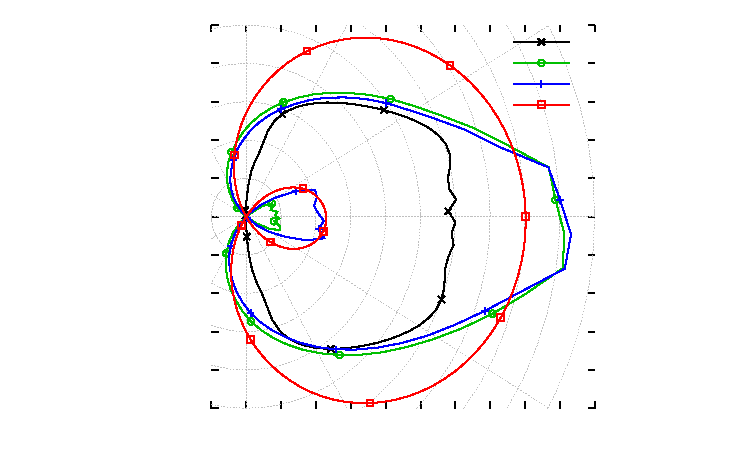
\includegraphics{/Users/seth/_thesis/figures/crashpipe2b/intens-x1-t1/intensity-x1-t1.pdf}}%
    \gplfronttext
  \end{picture}%
\endgroup

  \caption[Solution error (absolute volume-weighted 2-norm) in the
  finite difference discretization schemes.]{Solution error (absolute
  volume-weighted 2-norm) in the finite difference discretization schemes. The
  slopes of $\Delta_x^{2}$, $\Delta_x^{1.5}$, and
  $\Delta_x$, respectively.}
  \label{fig:manuConvergence}
\end{figure}

\begin{figure}[htb]
  \centering
  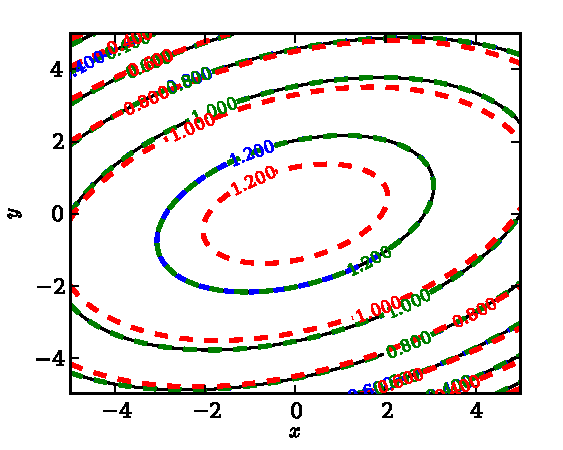
\includegraphics{manufactured/offdiag-contours}
  \caption[Solution contours for the manufactured solutions test.]{
  Solution contours for the manufactured solutions test. The red dashed line is
  the Diagonal scheme, the blue dashed line is the Gol'din scheme, cyan and green
  are the nine-point schemes, and the thin black line is the analytic solution.}
  \label{fig:manuSolution}
\end{figure}

\subsection{Transport discretization}

%%%%%%%%%%%%%%%%%%%%%%%%%%%%%%%%%%%%%%%%%%%%%%%%%%%%%%%%%%%%%%%%%%%%%%%%%%%%%%%%
\section{Flatland boundary conditions}

\begin{table}[htb]
  \centering
  \begin{tabular}{ccc}
\toprule
    Distribution & 1-D & Flatland
\\ \midrule
Isotropic & $I(\mu) = \frac{1}{2}$ & $I(\omega) = \frac{\pi}{2}$
\\
Normal & $I(\mu) = \delta(\mu-1)$ & $I(\omega) = \delta(\omega-\pi/2)$
\\
Grazing & $I(\mu) = \delta(\mu-0.1)$ & $I(\omega) = \delta(\omega-\sin\inv.1)$
\\ \bottomrule
  \end{tabular}
  \caption{Angular distributions used in boundary condition tests.}
  \label{tab:angularDistributions}
\end{table}

As a test problem, we consider a homogeneous flatland problem with a
total cross section $\sigma=1$ and scattering ratio $c=0.99$. It lives on the
domain $0 \le x \le 2$, $0 \le y \le 10$, with reflecting boundaries on the left,
right, and top sides. The bottom side has a specified boundary
condition with unit incident current, and we consider three different angular
distributions.

The first distribution is isotropic, $\psi^b(\omega) = \frac{1}{2}$. The second
is a normally incident flux, with all particles entering
perpendicular to the surface, $\psi^b(\omega) = \delta(\omega -
\frac{\pi}{2})$. The third incident distribution is at a grazing angle, with 
$\psi^b(\omega) = 10 \delta(\omega - \sin^{-1}.1)$.
These are the same angular distributions used in a boundary matching analysis
in \cite{Dav2006}.

Figure~\ref{fig:isotropic} shows a line-out of the scalar flux $\phi_0$ along
$x=1$ for an isotropic incident source. Because the left-hand sides of
Eqs.~\eqref{eq:flatlandDiffusionMarshak} and~\eqref{eq:flatlandDiffusionVarBc} are the same, the
differences in the solution are only due to the slightly different
extrapolation distance.

However, for the highly anisotropic normal and grazing cases,
Figs.~\ref{fig:delta} and~\ref{fig:grazing}, the Marshak boundary fails to
limit to the transport solution outside of the boundary layer. As
expected, the variational boundary condition does a much better job of
approximating the interior solution of the scalar flux.

\begin{figure}[htb!]
  \centering\small
  \hspace{-.5in}
  % GNUPLOT: LaTeX picture with Postscript
\begingroup
  \makeatletter
  \providecommand\color[2][]{%
    \GenericError{(gnuplot) \space\space\space\@spaces}{%
      Package color not loaded in conjunction with
      terminal option `colourtext'%
    }{See the gnuplot documentation for explanation.%
    }{Either use 'blacktext' in gnuplot or load the package
      color.sty in LaTeX.}%
    \renewcommand\color[2][]{}%
  }%
  \providecommand\includegraphics[2][]{%
    \GenericError{(gnuplot) \space\space\space\@spaces}{%
      Package graphicx or graphics not loaded%
    }{See the gnuplot documentation for explanation.%
    }{The gnuplot epslatex terminal needs graphicx.sty or graphics.sty.}%
    \renewcommand\includegraphics[2][]{}%
  }%
  \providecommand\rotatebox[2]{#2}%
  \@ifundefined{ifGPcolor}{%
    \newif\ifGPcolor
    \GPcolortrue
  }{}%
  \@ifundefined{ifGPblacktext}{%
    \newif\ifGPblacktext
    \GPblacktexttrue
  }{}%
  % define a \g@addto@macro without @ in the name:
  \let\gplgaddtomacro\g@addto@macro
  % define empty templates for all commands taking text:
  \gdef\gplbacktext{}%
  \gdef\gplfronttext{}%
  \makeatother
  \ifGPblacktext
    % no textcolor at all
    \def\colorrgb#1{}%
    \def\colorgray#1{}%
  \else
    % gray or color?
    \ifGPcolor
      \def\colorrgb#1{\color[rgb]{#1}}%
      \def\colorgray#1{\color[gray]{#1}}%
      \expandafter\def\csname LTw\endcsname{\color{white}}%
      \expandafter\def\csname LTb\endcsname{\color{black}}%
      \expandafter\def\csname LTa\endcsname{\color{black}}%
      \expandafter\def\csname LT0\endcsname{\color[rgb]{1,0,0}}%
      \expandafter\def\csname LT1\endcsname{\color[rgb]{0,1,0}}%
      \expandafter\def\csname LT2\endcsname{\color[rgb]{0,0,1}}%
      \expandafter\def\csname LT3\endcsname{\color[rgb]{1,0,1}}%
      \expandafter\def\csname LT4\endcsname{\color[rgb]{0,1,1}}%
      \expandafter\def\csname LT5\endcsname{\color[rgb]{1,1,0}}%
      \expandafter\def\csname LT6\endcsname{\color[rgb]{0,0,0}}%
      \expandafter\def\csname LT7\endcsname{\color[rgb]{1,0.3,0}}%
      \expandafter\def\csname LT8\endcsname{\color[rgb]{0.5,0.5,0.5}}%
    \else
      % gray
      \def\colorrgb#1{\color{black}}%
      \def\colorgray#1{\color[gray]{#1}}%
      \expandafter\def\csname LTw\endcsname{\color{white}}%
      \expandafter\def\csname LTb\endcsname{\color{black}}%
      \expandafter\def\csname LTa\endcsname{\color{black}}%
      \expandafter\def\csname LT0\endcsname{\color{black}}%
      \expandafter\def\csname LT1\endcsname{\color{black}}%
      \expandafter\def\csname LT2\endcsname{\color{black}}%
      \expandafter\def\csname LT3\endcsname{\color{black}}%
      \expandafter\def\csname LT4\endcsname{\color{black}}%
      \expandafter\def\csname LT5\endcsname{\color{black}}%
      \expandafter\def\csname LT6\endcsname{\color{black}}%
      \expandafter\def\csname LT7\endcsname{\color{black}}%
      \expandafter\def\csname LT8\endcsname{\color{black}}%
    \fi
  \fi
  \setlength{\unitlength}{0.0500bp}%
  \begin{picture}(7200.00,4320.00)%
    \gplgaddtomacro\gplbacktext{%
      \csname LTb\endcsname%
      \put(1910,400){\makebox(0,0)[r]{\strut{} 0.1}}%
      \put(1910,768){\makebox(0,0)[r]{\strut{} 0.08}}%
      \put(1910,1136){\makebox(0,0)[r]{\strut{} 0.06}}%
      \put(1910,1504){\makebox(0,0)[r]{\strut{} 0.04}}%
      \put(1910,1872){\makebox(0,0)[r]{\strut{} 0.02}}%
      \put(1910,2240){\makebox(0,0)[r]{\strut{} 0}}%
      \put(1910,2607){\makebox(0,0)[r]{\strut{} 0.02}}%
      \put(1910,2975){\makebox(0,0)[r]{\strut{} 0.04}}%
      \put(1910,3343){\makebox(0,0)[r]{\strut{} 0.06}}%
      \put(1910,3711){\makebox(0,0)[r]{\strut{} 0.08}}%
      \put(1910,4079){\makebox(0,0)[r]{\strut{} 0.1}}%
      \csname LTb\endcsname%
      \put(2030,200){\makebox(0,0){\strut{} 0.02}}%
      \csname LTb\endcsname%
      \put(2364,200){\makebox(0,0){\strut{} 0}}%
      \csname LTb\endcsname%
      \put(2699,200){\makebox(0,0){\strut{} 0.02}}%
      \csname LTb\endcsname%
      \put(3033,200){\makebox(0,0){\strut{} 0.04}}%
      \csname LTb\endcsname%
      \put(3368,200){\makebox(0,0){\strut{} 0.06}}%
      \csname LTb\endcsname%
      \put(3702,200){\makebox(0,0){\strut{} 0.08}}%
      \csname LTb\endcsname%
      \put(4037,200){\makebox(0,0){\strut{} 0.1}}%
      \csname LTb\endcsname%
      \put(4371,200){\makebox(0,0){\strut{} 0.12}}%
      \csname LTb\endcsname%
      \put(4706,200){\makebox(0,0){\strut{} 0.14}}%
      \csname LTb\endcsname%
      \put(5040,200){\makebox(0,0){\strut{} 0.16}}%
      \csname LTb\endcsname%
      \put(5375,200){\makebox(0,0){\strut{} 0.18}}%
      \csname LTb\endcsname%
      \put(5709,200){\makebox(0,0){\strut{} 0.2}}%
      \csname LTb\endcsname%
      \put(1330,2239){\rotatebox{-270}{\makebox(0,0){\strut{}x1 center $(1.01,3.5)$}}}%
    }%
    \gplgaddtomacro\gplfronttext{%
      \csname LTb\endcsname%
      \put(4806,3916){\makebox(0,0)[r]{\strut{}S$_{128}$}}%
      \csname LTb\endcsname%
      \put(4806,3716){\makebox(0,0)[r]{\strut{}FLAD$_{64}$}}%
      \csname LTb\endcsname%
      \put(4806,3516){\makebox(0,0)[r]{\strut{}AD$_{64}$}}%
      \csname LTb\endcsname%
      \put(4806,3316){\makebox(0,0)[r]{\strut{}FLD}}%
    }%
    \gplbacktext
    \put(0,0){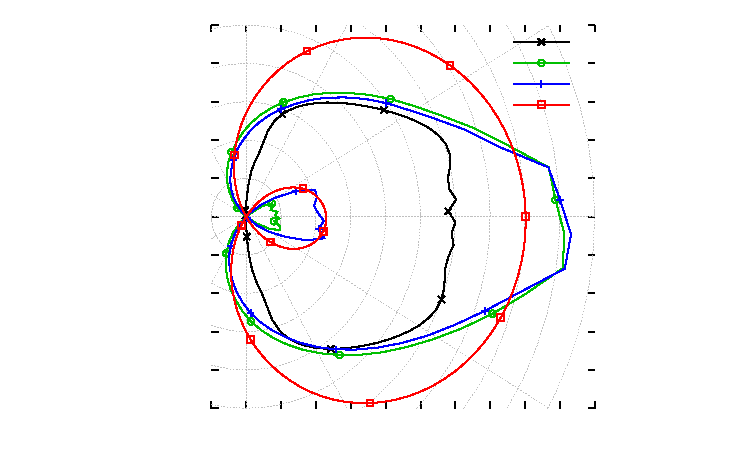
\includegraphics{/Users/seth/_thesis/figures/crashpipe2b/intens-x1-t1/intensity-x1-t1.pdf}}%
    \gplfronttext
  \end{picture}%
\endgroup

  \hspace{-.5in}
  \caption{Scalar flux with an isotropic boundary condition in a homogeneous
  flatland problem.}
  \label{fig:isotropic}
\end{figure}

\begin{figure}[htb!]
  \centering\small
  \hspace{-.5in}
  % GNUPLOT: LaTeX picture with Postscript
\begingroup
  \makeatletter
  \providecommand\color[2][]{%
    \GenericError{(gnuplot) \space\space\space\@spaces}{%
      Package color not loaded in conjunction with
      terminal option `colourtext'%
    }{See the gnuplot documentation for explanation.%
    }{Either use 'blacktext' in gnuplot or load the package
      color.sty in LaTeX.}%
    \renewcommand\color[2][]{}%
  }%
  \providecommand\includegraphics[2][]{%
    \GenericError{(gnuplot) \space\space\space\@spaces}{%
      Package graphicx or graphics not loaded%
    }{See the gnuplot documentation for explanation.%
    }{The gnuplot epslatex terminal needs graphicx.sty or graphics.sty.}%
    \renewcommand\includegraphics[2][]{}%
  }%
  \providecommand\rotatebox[2]{#2}%
  \@ifundefined{ifGPcolor}{%
    \newif\ifGPcolor
    \GPcolortrue
  }{}%
  \@ifundefined{ifGPblacktext}{%
    \newif\ifGPblacktext
    \GPblacktexttrue
  }{}%
  % define a \g@addto@macro without @ in the name:
  \let\gplgaddtomacro\g@addto@macro
  % define empty templates for all commands taking text:
  \gdef\gplbacktext{}%
  \gdef\gplfronttext{}%
  \makeatother
  \ifGPblacktext
    % no textcolor at all
    \def\colorrgb#1{}%
    \def\colorgray#1{}%
  \else
    % gray or color?
    \ifGPcolor
      \def\colorrgb#1{\color[rgb]{#1}}%
      \def\colorgray#1{\color[gray]{#1}}%
      \expandafter\def\csname LTw\endcsname{\color{white}}%
      \expandafter\def\csname LTb\endcsname{\color{black}}%
      \expandafter\def\csname LTa\endcsname{\color{black}}%
      \expandafter\def\csname LT0\endcsname{\color[rgb]{1,0,0}}%
      \expandafter\def\csname LT1\endcsname{\color[rgb]{0,1,0}}%
      \expandafter\def\csname LT2\endcsname{\color[rgb]{0,0,1}}%
      \expandafter\def\csname LT3\endcsname{\color[rgb]{1,0,1}}%
      \expandafter\def\csname LT4\endcsname{\color[rgb]{0,1,1}}%
      \expandafter\def\csname LT5\endcsname{\color[rgb]{1,1,0}}%
      \expandafter\def\csname LT6\endcsname{\color[rgb]{0,0,0}}%
      \expandafter\def\csname LT7\endcsname{\color[rgb]{1,0.3,0}}%
      \expandafter\def\csname LT8\endcsname{\color[rgb]{0.5,0.5,0.5}}%
    \else
      % gray
      \def\colorrgb#1{\color{black}}%
      \def\colorgray#1{\color[gray]{#1}}%
      \expandafter\def\csname LTw\endcsname{\color{white}}%
      \expandafter\def\csname LTb\endcsname{\color{black}}%
      \expandafter\def\csname LTa\endcsname{\color{black}}%
      \expandafter\def\csname LT0\endcsname{\color{black}}%
      \expandafter\def\csname LT1\endcsname{\color{black}}%
      \expandafter\def\csname LT2\endcsname{\color{black}}%
      \expandafter\def\csname LT3\endcsname{\color{black}}%
      \expandafter\def\csname LT4\endcsname{\color{black}}%
      \expandafter\def\csname LT5\endcsname{\color{black}}%
      \expandafter\def\csname LT6\endcsname{\color{black}}%
      \expandafter\def\csname LT7\endcsname{\color{black}}%
      \expandafter\def\csname LT8\endcsname{\color{black}}%
    \fi
  \fi
  \setlength{\unitlength}{0.0500bp}%
  \begin{picture}(7200.00,4320.00)%
    \gplgaddtomacro\gplbacktext{%
      \csname LTb\endcsname%
      \put(1910,400){\makebox(0,0)[r]{\strut{} 0.1}}%
      \put(1910,768){\makebox(0,0)[r]{\strut{} 0.08}}%
      \put(1910,1136){\makebox(0,0)[r]{\strut{} 0.06}}%
      \put(1910,1504){\makebox(0,0)[r]{\strut{} 0.04}}%
      \put(1910,1872){\makebox(0,0)[r]{\strut{} 0.02}}%
      \put(1910,2240){\makebox(0,0)[r]{\strut{} 0}}%
      \put(1910,2607){\makebox(0,0)[r]{\strut{} 0.02}}%
      \put(1910,2975){\makebox(0,0)[r]{\strut{} 0.04}}%
      \put(1910,3343){\makebox(0,0)[r]{\strut{} 0.06}}%
      \put(1910,3711){\makebox(0,0)[r]{\strut{} 0.08}}%
      \put(1910,4079){\makebox(0,0)[r]{\strut{} 0.1}}%
      \csname LTb\endcsname%
      \put(2030,200){\makebox(0,0){\strut{} 0.02}}%
      \csname LTb\endcsname%
      \put(2364,200){\makebox(0,0){\strut{} 0}}%
      \csname LTb\endcsname%
      \put(2699,200){\makebox(0,0){\strut{} 0.02}}%
      \csname LTb\endcsname%
      \put(3033,200){\makebox(0,0){\strut{} 0.04}}%
      \csname LTb\endcsname%
      \put(3368,200){\makebox(0,0){\strut{} 0.06}}%
      \csname LTb\endcsname%
      \put(3702,200){\makebox(0,0){\strut{} 0.08}}%
      \csname LTb\endcsname%
      \put(4037,200){\makebox(0,0){\strut{} 0.1}}%
      \csname LTb\endcsname%
      \put(4371,200){\makebox(0,0){\strut{} 0.12}}%
      \csname LTb\endcsname%
      \put(4706,200){\makebox(0,0){\strut{} 0.14}}%
      \csname LTb\endcsname%
      \put(5040,200){\makebox(0,0){\strut{} 0.16}}%
      \csname LTb\endcsname%
      \put(5375,200){\makebox(0,0){\strut{} 0.18}}%
      \csname LTb\endcsname%
      \put(5709,200){\makebox(0,0){\strut{} 0.2}}%
      \csname LTb\endcsname%
      \put(1330,2239){\rotatebox{-270}{\makebox(0,0){\strut{}x1 center $(1.01,3.5)$}}}%
    }%
    \gplgaddtomacro\gplfronttext{%
      \csname LTb\endcsname%
      \put(4806,3916){\makebox(0,0)[r]{\strut{}S$_{128}$}}%
      \csname LTb\endcsname%
      \put(4806,3716){\makebox(0,0)[r]{\strut{}FLAD$_{64}$}}%
      \csname LTb\endcsname%
      \put(4806,3516){\makebox(0,0)[r]{\strut{}AD$_{64}$}}%
      \csname LTb\endcsname%
      \put(4806,3316){\makebox(0,0)[r]{\strut{}FLD}}%
    }%
    \gplbacktext
    \put(0,0){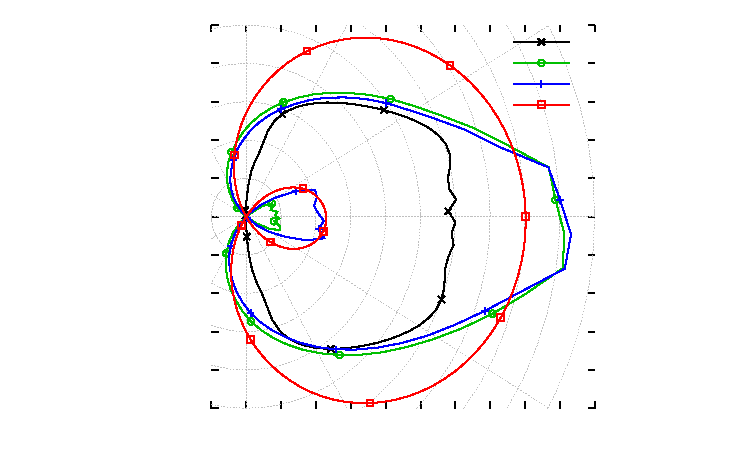
\includegraphics{/Users/seth/_thesis/figures/crashpipe2b/intens-x1-t1/intensity-x1-t1.pdf}}%
    \gplfronttext
  \end{picture}%
\endgroup

  \hspace{-.5in}
  \caption{Scalar flux with a normally incident boundary condition in a
  homogeneous flatland problem.}
  \label{fig:delta}
\end{figure}

\begin{figure}[htb!]
  \centering\small
  \hspace{-.5in}
  % GNUPLOT: LaTeX picture with Postscript
\begingroup
  \makeatletter
  \providecommand\color[2][]{%
    \GenericError{(gnuplot) \space\space\space\@spaces}{%
      Package color not loaded in conjunction with
      terminal option `colourtext'%
    }{See the gnuplot documentation for explanation.%
    }{Either use 'blacktext' in gnuplot or load the package
      color.sty in LaTeX.}%
    \renewcommand\color[2][]{}%
  }%
  \providecommand\includegraphics[2][]{%
    \GenericError{(gnuplot) \space\space\space\@spaces}{%
      Package graphicx or graphics not loaded%
    }{See the gnuplot documentation for explanation.%
    }{The gnuplot epslatex terminal needs graphicx.sty or graphics.sty.}%
    \renewcommand\includegraphics[2][]{}%
  }%
  \providecommand\rotatebox[2]{#2}%
  \@ifundefined{ifGPcolor}{%
    \newif\ifGPcolor
    \GPcolortrue
  }{}%
  \@ifundefined{ifGPblacktext}{%
    \newif\ifGPblacktext
    \GPblacktexttrue
  }{}%
  % define a \g@addto@macro without @ in the name:
  \let\gplgaddtomacro\g@addto@macro
  % define empty templates for all commands taking text:
  \gdef\gplbacktext{}%
  \gdef\gplfronttext{}%
  \makeatother
  \ifGPblacktext
    % no textcolor at all
    \def\colorrgb#1{}%
    \def\colorgray#1{}%
  \else
    % gray or color?
    \ifGPcolor
      \def\colorrgb#1{\color[rgb]{#1}}%
      \def\colorgray#1{\color[gray]{#1}}%
      \expandafter\def\csname LTw\endcsname{\color{white}}%
      \expandafter\def\csname LTb\endcsname{\color{black}}%
      \expandafter\def\csname LTa\endcsname{\color{black}}%
      \expandafter\def\csname LT0\endcsname{\color[rgb]{1,0,0}}%
      \expandafter\def\csname LT1\endcsname{\color[rgb]{0,1,0}}%
      \expandafter\def\csname LT2\endcsname{\color[rgb]{0,0,1}}%
      \expandafter\def\csname LT3\endcsname{\color[rgb]{1,0,1}}%
      \expandafter\def\csname LT4\endcsname{\color[rgb]{0,1,1}}%
      \expandafter\def\csname LT5\endcsname{\color[rgb]{1,1,0}}%
      \expandafter\def\csname LT6\endcsname{\color[rgb]{0,0,0}}%
      \expandafter\def\csname LT7\endcsname{\color[rgb]{1,0.3,0}}%
      \expandafter\def\csname LT8\endcsname{\color[rgb]{0.5,0.5,0.5}}%
    \else
      % gray
      \def\colorrgb#1{\color{black}}%
      \def\colorgray#1{\color[gray]{#1}}%
      \expandafter\def\csname LTw\endcsname{\color{white}}%
      \expandafter\def\csname LTb\endcsname{\color{black}}%
      \expandafter\def\csname LTa\endcsname{\color{black}}%
      \expandafter\def\csname LT0\endcsname{\color{black}}%
      \expandafter\def\csname LT1\endcsname{\color{black}}%
      \expandafter\def\csname LT2\endcsname{\color{black}}%
      \expandafter\def\csname LT3\endcsname{\color{black}}%
      \expandafter\def\csname LT4\endcsname{\color{black}}%
      \expandafter\def\csname LT5\endcsname{\color{black}}%
      \expandafter\def\csname LT6\endcsname{\color{black}}%
      \expandafter\def\csname LT7\endcsname{\color{black}}%
      \expandafter\def\csname LT8\endcsname{\color{black}}%
    \fi
  \fi
  \setlength{\unitlength}{0.0500bp}%
  \begin{picture}(7200.00,4320.00)%
    \gplgaddtomacro\gplbacktext{%
      \csname LTb\endcsname%
      \put(1910,400){\makebox(0,0)[r]{\strut{} 0.1}}%
      \put(1910,768){\makebox(0,0)[r]{\strut{} 0.08}}%
      \put(1910,1136){\makebox(0,0)[r]{\strut{} 0.06}}%
      \put(1910,1504){\makebox(0,0)[r]{\strut{} 0.04}}%
      \put(1910,1872){\makebox(0,0)[r]{\strut{} 0.02}}%
      \put(1910,2240){\makebox(0,0)[r]{\strut{} 0}}%
      \put(1910,2607){\makebox(0,0)[r]{\strut{} 0.02}}%
      \put(1910,2975){\makebox(0,0)[r]{\strut{} 0.04}}%
      \put(1910,3343){\makebox(0,0)[r]{\strut{} 0.06}}%
      \put(1910,3711){\makebox(0,0)[r]{\strut{} 0.08}}%
      \put(1910,4079){\makebox(0,0)[r]{\strut{} 0.1}}%
      \csname LTb\endcsname%
      \put(2030,200){\makebox(0,0){\strut{} 0.02}}%
      \csname LTb\endcsname%
      \put(2364,200){\makebox(0,0){\strut{} 0}}%
      \csname LTb\endcsname%
      \put(2699,200){\makebox(0,0){\strut{} 0.02}}%
      \csname LTb\endcsname%
      \put(3033,200){\makebox(0,0){\strut{} 0.04}}%
      \csname LTb\endcsname%
      \put(3368,200){\makebox(0,0){\strut{} 0.06}}%
      \csname LTb\endcsname%
      \put(3702,200){\makebox(0,0){\strut{} 0.08}}%
      \csname LTb\endcsname%
      \put(4037,200){\makebox(0,0){\strut{} 0.1}}%
      \csname LTb\endcsname%
      \put(4371,200){\makebox(0,0){\strut{} 0.12}}%
      \csname LTb\endcsname%
      \put(4706,200){\makebox(0,0){\strut{} 0.14}}%
      \csname LTb\endcsname%
      \put(5040,200){\makebox(0,0){\strut{} 0.16}}%
      \csname LTb\endcsname%
      \put(5375,200){\makebox(0,0){\strut{} 0.18}}%
      \csname LTb\endcsname%
      \put(5709,200){\makebox(0,0){\strut{} 0.2}}%
      \csname LTb\endcsname%
      \put(1330,2239){\rotatebox{-270}{\makebox(0,0){\strut{}x1 center $(1.01,3.5)$}}}%
    }%
    \gplgaddtomacro\gplfronttext{%
      \csname LTb\endcsname%
      \put(4806,3916){\makebox(0,0)[r]{\strut{}S$_{128}$}}%
      \csname LTb\endcsname%
      \put(4806,3716){\makebox(0,0)[r]{\strut{}FLAD$_{64}$}}%
      \csname LTb\endcsname%
      \put(4806,3516){\makebox(0,0)[r]{\strut{}AD$_{64}$}}%
      \csname LTb\endcsname%
      \put(4806,3316){\makebox(0,0)[r]{\strut{}FLD}}%
    }%
    \gplbacktext
    \put(0,0){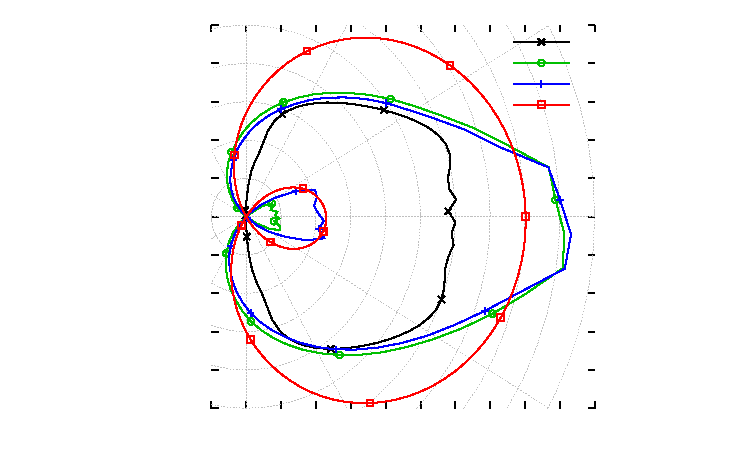
\includegraphics{/Users/seth/_thesis/figures/crashpipe2b/intens-x1-t1/intensity-x1-t1.pdf}}%
    \gplfronttext
  \end{picture}%
\endgroup

  \hspace{-.5in}
  \caption{Scalar flux with a grazing boundary condition in a homogeneous
  flatland problem.}
  \label{fig:grazing}
\end{figure}

%%%%%%%%%%%%%%%%%%%%%%%%%%%%%%%%%%%%%%%%%%%%%%%%%%%%%%%%%%%%%%%%%%%%%%%%%%%%%%%%
\section{Anisotropic diffusion boundary conditions}

%%%%%%%%%%%%%%%%%%%%%%%%%%%%%%%%%%%%%%%%%%%%%%%%%%%%%%%%%%%%%%%%%%%%%%%%%%%%%%%%
\subsection{Steady-state flatland channel}
As a test problem, we consider a diffusive medium in flatland on
the domain $0
\le x \le 5$ and $0 \le y \le 10$, with a channel of unit width running
vertically through the middle. The diffusive region has $\sigma=1$ and
$\sigma_s=0.99$, and the channel has $\sigma=0.01$ and $\sigma_s=0.0099$. It has
reflecting boundaries on the top, left, and right sides, and an incident
boundary condition on the bottom. The geometry and cross sections are similar to Larsen
and Trahan's VHTR problem \cite{Lar2009c}.

We compare the AD method using three different boundary conditions for $f$ on
the bottom surface: a reflecting boundary, a white boundary, and a vacuum
boundary. The vacuum boundary is not consistent with our theory but
is shown to gauge how much $\phi$ is affected by the choice of $\zeta$.

Figure~\ref{fig:bcChannelIsotropic} shows a line-out of the scalar flux
$\phi(2.5,y)$, along the center
of the channel. Standard diffusion fails because $\sigma=0.01$ leads to a very
large diffusion coefficient, resulting in a nearly constant solution inside the
channel. Anisotropic diffusion performs exceedingly well, and curiously the
white boundary gives a better result than the reflecting boundary.

\begin{figure}[htb]
  \centering\small
  \hspace{-.5in}
  % GNUPLOT: LaTeX picture with Postscript
\begingroup
  \makeatletter
  \providecommand\color[2][]{%
    \GenericError{(gnuplot) \space\space\space\@spaces}{%
      Package color not loaded in conjunction with
      terminal option `colourtext'%
    }{See the gnuplot documentation for explanation.%
    }{Either use 'blacktext' in gnuplot or load the package
      color.sty in LaTeX.}%
    \renewcommand\color[2][]{}%
  }%
  \providecommand\includegraphics[2][]{%
    \GenericError{(gnuplot) \space\space\space\@spaces}{%
      Package graphicx or graphics not loaded%
    }{See the gnuplot documentation for explanation.%
    }{The gnuplot epslatex terminal needs graphicx.sty or graphics.sty.}%
    \renewcommand\includegraphics[2][]{}%
  }%
  \providecommand\rotatebox[2]{#2}%
  \@ifundefined{ifGPcolor}{%
    \newif\ifGPcolor
    \GPcolortrue
  }{}%
  \@ifundefined{ifGPblacktext}{%
    \newif\ifGPblacktext
    \GPblacktexttrue
  }{}%
  % define a \g@addto@macro without @ in the name:
  \let\gplgaddtomacro\g@addto@macro
  % define empty templates for all commands taking text:
  \gdef\gplbacktext{}%
  \gdef\gplfronttext{}%
  \makeatother
  \ifGPblacktext
    % no textcolor at all
    \def\colorrgb#1{}%
    \def\colorgray#1{}%
  \else
    % gray or color?
    \ifGPcolor
      \def\colorrgb#1{\color[rgb]{#1}}%
      \def\colorgray#1{\color[gray]{#1}}%
      \expandafter\def\csname LTw\endcsname{\color{white}}%
      \expandafter\def\csname LTb\endcsname{\color{black}}%
      \expandafter\def\csname LTa\endcsname{\color{black}}%
      \expandafter\def\csname LT0\endcsname{\color[rgb]{1,0,0}}%
      \expandafter\def\csname LT1\endcsname{\color[rgb]{0,1,0}}%
      \expandafter\def\csname LT2\endcsname{\color[rgb]{0,0,1}}%
      \expandafter\def\csname LT3\endcsname{\color[rgb]{1,0,1}}%
      \expandafter\def\csname LT4\endcsname{\color[rgb]{0,1,1}}%
      \expandafter\def\csname LT5\endcsname{\color[rgb]{1,1,0}}%
      \expandafter\def\csname LT6\endcsname{\color[rgb]{0,0,0}}%
      \expandafter\def\csname LT7\endcsname{\color[rgb]{1,0.3,0}}%
      \expandafter\def\csname LT8\endcsname{\color[rgb]{0.5,0.5,0.5}}%
    \else
      % gray
      \def\colorrgb#1{\color{black}}%
      \def\colorgray#1{\color[gray]{#1}}%
      \expandafter\def\csname LTw\endcsname{\color{white}}%
      \expandafter\def\csname LTb\endcsname{\color{black}}%
      \expandafter\def\csname LTa\endcsname{\color{black}}%
      \expandafter\def\csname LT0\endcsname{\color{black}}%
      \expandafter\def\csname LT1\endcsname{\color{black}}%
      \expandafter\def\csname LT2\endcsname{\color{black}}%
      \expandafter\def\csname LT3\endcsname{\color{black}}%
      \expandafter\def\csname LT4\endcsname{\color{black}}%
      \expandafter\def\csname LT5\endcsname{\color{black}}%
      \expandafter\def\csname LT6\endcsname{\color{black}}%
      \expandafter\def\csname LT7\endcsname{\color{black}}%
      \expandafter\def\csname LT8\endcsname{\color{black}}%
    \fi
  \fi
  \setlength{\unitlength}{0.0500bp}%
  \begin{picture}(7200.00,4320.00)%
    \gplgaddtomacro\gplbacktext{%
      \csname LTb\endcsname%
      \put(1910,400){\makebox(0,0)[r]{\strut{} 0.1}}%
      \put(1910,768){\makebox(0,0)[r]{\strut{} 0.08}}%
      \put(1910,1136){\makebox(0,0)[r]{\strut{} 0.06}}%
      \put(1910,1504){\makebox(0,0)[r]{\strut{} 0.04}}%
      \put(1910,1872){\makebox(0,0)[r]{\strut{} 0.02}}%
      \put(1910,2240){\makebox(0,0)[r]{\strut{} 0}}%
      \put(1910,2607){\makebox(0,0)[r]{\strut{} 0.02}}%
      \put(1910,2975){\makebox(0,0)[r]{\strut{} 0.04}}%
      \put(1910,3343){\makebox(0,0)[r]{\strut{} 0.06}}%
      \put(1910,3711){\makebox(0,0)[r]{\strut{} 0.08}}%
      \put(1910,4079){\makebox(0,0)[r]{\strut{} 0.1}}%
      \csname LTb\endcsname%
      \put(2030,200){\makebox(0,0){\strut{} 0.02}}%
      \csname LTb\endcsname%
      \put(2364,200){\makebox(0,0){\strut{} 0}}%
      \csname LTb\endcsname%
      \put(2699,200){\makebox(0,0){\strut{} 0.02}}%
      \csname LTb\endcsname%
      \put(3033,200){\makebox(0,0){\strut{} 0.04}}%
      \csname LTb\endcsname%
      \put(3368,200){\makebox(0,0){\strut{} 0.06}}%
      \csname LTb\endcsname%
      \put(3702,200){\makebox(0,0){\strut{} 0.08}}%
      \csname LTb\endcsname%
      \put(4037,200){\makebox(0,0){\strut{} 0.1}}%
      \csname LTb\endcsname%
      \put(4371,200){\makebox(0,0){\strut{} 0.12}}%
      \csname LTb\endcsname%
      \put(4706,200){\makebox(0,0){\strut{} 0.14}}%
      \csname LTb\endcsname%
      \put(5040,200){\makebox(0,0){\strut{} 0.16}}%
      \csname LTb\endcsname%
      \put(5375,200){\makebox(0,0){\strut{} 0.18}}%
      \csname LTb\endcsname%
      \put(5709,200){\makebox(0,0){\strut{} 0.2}}%
      \csname LTb\endcsname%
      \put(1330,2239){\rotatebox{-270}{\makebox(0,0){\strut{}x1 center $(1.01,3.5)$}}}%
    }%
    \gplgaddtomacro\gplfronttext{%
      \csname LTb\endcsname%
      \put(4806,3916){\makebox(0,0)[r]{\strut{}S$_{128}$}}%
      \csname LTb\endcsname%
      \put(4806,3716){\makebox(0,0)[r]{\strut{}FLAD$_{64}$}}%
      \csname LTb\endcsname%
      \put(4806,3516){\makebox(0,0)[r]{\strut{}AD$_{64}$}}%
      \csname LTb\endcsname%
      \put(4806,3316){\makebox(0,0)[r]{\strut{}FLD}}%
    }%
    \gplbacktext
    \put(0,0){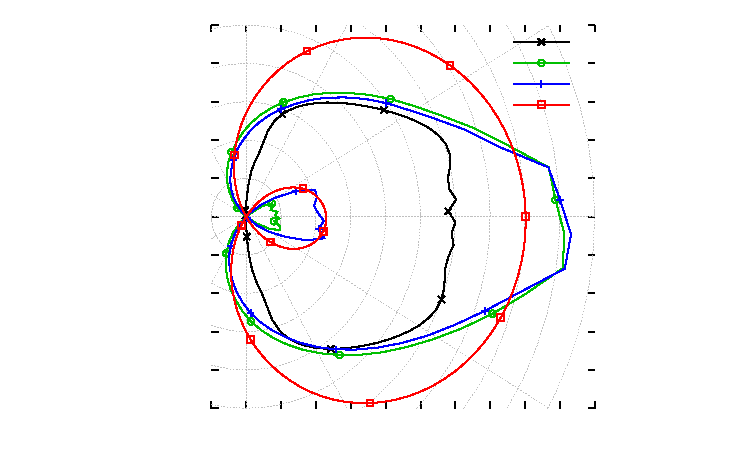
\includegraphics{/Users/seth/_thesis/figures/crashpipe2b/intens-x1-t1/intensity-x1-t1.pdf}}%
    \gplfronttext
  \end{picture}%
\endgroup

  \hspace{-.5in}
  \caption{Scalar flux along the centerline of the channel with an isotropic
  boundary condition at $y=0$.}
  \label{fig:bcChannelIsotropic}
\end{figure}

\begin{figure}[htb]
  \centering\small
  \hspace{-.5in}
  % GNUPLOT: LaTeX picture with Postscript
\begingroup
  \makeatletter
  \providecommand\color[2][]{%
    \GenericError{(gnuplot) \space\space\space\@spaces}{%
      Package color not loaded in conjunction with
      terminal option `colourtext'%
    }{See the gnuplot documentation for explanation.%
    }{Either use 'blacktext' in gnuplot or load the package
      color.sty in LaTeX.}%
    \renewcommand\color[2][]{}%
  }%
  \providecommand\includegraphics[2][]{%
    \GenericError{(gnuplot) \space\space\space\@spaces}{%
      Package graphicx or graphics not loaded%
    }{See the gnuplot documentation for explanation.%
    }{The gnuplot epslatex terminal needs graphicx.sty or graphics.sty.}%
    \renewcommand\includegraphics[2][]{}%
  }%
  \providecommand\rotatebox[2]{#2}%
  \@ifundefined{ifGPcolor}{%
    \newif\ifGPcolor
    \GPcolortrue
  }{}%
  \@ifundefined{ifGPblacktext}{%
    \newif\ifGPblacktext
    \GPblacktexttrue
  }{}%
  % define a \g@addto@macro without @ in the name:
  \let\gplgaddtomacro\g@addto@macro
  % define empty templates for all commands taking text:
  \gdef\gplbacktext{}%
  \gdef\gplfronttext{}%
  \makeatother
  \ifGPblacktext
    % no textcolor at all
    \def\colorrgb#1{}%
    \def\colorgray#1{}%
  \else
    % gray or color?
    \ifGPcolor
      \def\colorrgb#1{\color[rgb]{#1}}%
      \def\colorgray#1{\color[gray]{#1}}%
      \expandafter\def\csname LTw\endcsname{\color{white}}%
      \expandafter\def\csname LTb\endcsname{\color{black}}%
      \expandafter\def\csname LTa\endcsname{\color{black}}%
      \expandafter\def\csname LT0\endcsname{\color[rgb]{1,0,0}}%
      \expandafter\def\csname LT1\endcsname{\color[rgb]{0,1,0}}%
      \expandafter\def\csname LT2\endcsname{\color[rgb]{0,0,1}}%
      \expandafter\def\csname LT3\endcsname{\color[rgb]{1,0,1}}%
      \expandafter\def\csname LT4\endcsname{\color[rgb]{0,1,1}}%
      \expandafter\def\csname LT5\endcsname{\color[rgb]{1,1,0}}%
      \expandafter\def\csname LT6\endcsname{\color[rgb]{0,0,0}}%
      \expandafter\def\csname LT7\endcsname{\color[rgb]{1,0.3,0}}%
      \expandafter\def\csname LT8\endcsname{\color[rgb]{0.5,0.5,0.5}}%
    \else
      % gray
      \def\colorrgb#1{\color{black}}%
      \def\colorgray#1{\color[gray]{#1}}%
      \expandafter\def\csname LTw\endcsname{\color{white}}%
      \expandafter\def\csname LTb\endcsname{\color{black}}%
      \expandafter\def\csname LTa\endcsname{\color{black}}%
      \expandafter\def\csname LT0\endcsname{\color{black}}%
      \expandafter\def\csname LT1\endcsname{\color{black}}%
      \expandafter\def\csname LT2\endcsname{\color{black}}%
      \expandafter\def\csname LT3\endcsname{\color{black}}%
      \expandafter\def\csname LT4\endcsname{\color{black}}%
      \expandafter\def\csname LT5\endcsname{\color{black}}%
      \expandafter\def\csname LT6\endcsname{\color{black}}%
      \expandafter\def\csname LT7\endcsname{\color{black}}%
      \expandafter\def\csname LT8\endcsname{\color{black}}%
    \fi
  \fi
  \setlength{\unitlength}{0.0500bp}%
  \begin{picture}(7200.00,4320.00)%
    \gplgaddtomacro\gplbacktext{%
      \csname LTb\endcsname%
      \put(1910,400){\makebox(0,0)[r]{\strut{} 0.1}}%
      \put(1910,768){\makebox(0,0)[r]{\strut{} 0.08}}%
      \put(1910,1136){\makebox(0,0)[r]{\strut{} 0.06}}%
      \put(1910,1504){\makebox(0,0)[r]{\strut{} 0.04}}%
      \put(1910,1872){\makebox(0,0)[r]{\strut{} 0.02}}%
      \put(1910,2240){\makebox(0,0)[r]{\strut{} 0}}%
      \put(1910,2607){\makebox(0,0)[r]{\strut{} 0.02}}%
      \put(1910,2975){\makebox(0,0)[r]{\strut{} 0.04}}%
      \put(1910,3343){\makebox(0,0)[r]{\strut{} 0.06}}%
      \put(1910,3711){\makebox(0,0)[r]{\strut{} 0.08}}%
      \put(1910,4079){\makebox(0,0)[r]{\strut{} 0.1}}%
      \csname LTb\endcsname%
      \put(2030,200){\makebox(0,0){\strut{} 0.02}}%
      \csname LTb\endcsname%
      \put(2364,200){\makebox(0,0){\strut{} 0}}%
      \csname LTb\endcsname%
      \put(2699,200){\makebox(0,0){\strut{} 0.02}}%
      \csname LTb\endcsname%
      \put(3033,200){\makebox(0,0){\strut{} 0.04}}%
      \csname LTb\endcsname%
      \put(3368,200){\makebox(0,0){\strut{} 0.06}}%
      \csname LTb\endcsname%
      \put(3702,200){\makebox(0,0){\strut{} 0.08}}%
      \csname LTb\endcsname%
      \put(4037,200){\makebox(0,0){\strut{} 0.1}}%
      \csname LTb\endcsname%
      \put(4371,200){\makebox(0,0){\strut{} 0.12}}%
      \csname LTb\endcsname%
      \put(4706,200){\makebox(0,0){\strut{} 0.14}}%
      \csname LTb\endcsname%
      \put(5040,200){\makebox(0,0){\strut{} 0.16}}%
      \csname LTb\endcsname%
      \put(5375,200){\makebox(0,0){\strut{} 0.18}}%
      \csname LTb\endcsname%
      \put(5709,200){\makebox(0,0){\strut{} 0.2}}%
      \csname LTb\endcsname%
      \put(1330,2239){\rotatebox{-270}{\makebox(0,0){\strut{}x1 center $(1.01,3.5)$}}}%
    }%
    \gplgaddtomacro\gplfronttext{%
      \csname LTb\endcsname%
      \put(4806,3916){\makebox(0,0)[r]{\strut{}S$_{128}$}}%
      \csname LTb\endcsname%
      \put(4806,3716){\makebox(0,0)[r]{\strut{}FLAD$_{64}$}}%
      \csname LTb\endcsname%
      \put(4806,3516){\makebox(0,0)[r]{\strut{}AD$_{64}$}}%
      \csname LTb\endcsname%
      \put(4806,3316){\makebox(0,0)[r]{\strut{}FLD}}%
    }%
    \gplbacktext
    \put(0,0){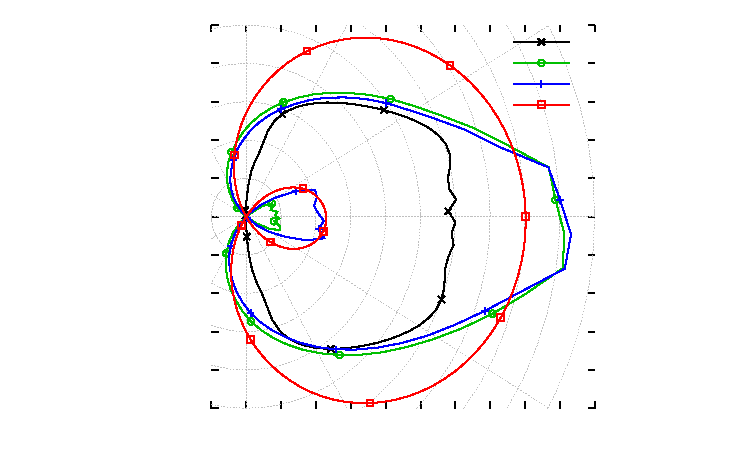
\includegraphics{/Users/seth/_thesis/figures/crashpipe2b/intens-x1-t1/intensity-x1-t1.pdf}}%
    \gplfronttext
  \end{picture}%
\endgroup

  \hspace{-.5in}
  \caption{Scalar flux along the centerline of the channel with a normal
  boundary condition at $y=0$.}
  \label{fig:bcChannelDelta}
\end{figure}

\begin{figure}[htb]
  \centering\small
  \hspace{-.5in}
  % GNUPLOT: LaTeX picture with Postscript
\begingroup
  \makeatletter
  \providecommand\color[2][]{%
    \GenericError{(gnuplot) \space\space\space\@spaces}{%
      Package color not loaded in conjunction with
      terminal option `colourtext'%
    }{See the gnuplot documentation for explanation.%
    }{Either use 'blacktext' in gnuplot or load the package
      color.sty in LaTeX.}%
    \renewcommand\color[2][]{}%
  }%
  \providecommand\includegraphics[2][]{%
    \GenericError{(gnuplot) \space\space\space\@spaces}{%
      Package graphicx or graphics not loaded%
    }{See the gnuplot documentation for explanation.%
    }{The gnuplot epslatex terminal needs graphicx.sty or graphics.sty.}%
    \renewcommand\includegraphics[2][]{}%
  }%
  \providecommand\rotatebox[2]{#2}%
  \@ifundefined{ifGPcolor}{%
    \newif\ifGPcolor
    \GPcolortrue
  }{}%
  \@ifundefined{ifGPblacktext}{%
    \newif\ifGPblacktext
    \GPblacktexttrue
  }{}%
  % define a \g@addto@macro without @ in the name:
  \let\gplgaddtomacro\g@addto@macro
  % define empty templates for all commands taking text:
  \gdef\gplbacktext{}%
  \gdef\gplfronttext{}%
  \makeatother
  \ifGPblacktext
    % no textcolor at all
    \def\colorrgb#1{}%
    \def\colorgray#1{}%
  \else
    % gray or color?
    \ifGPcolor
      \def\colorrgb#1{\color[rgb]{#1}}%
      \def\colorgray#1{\color[gray]{#1}}%
      \expandafter\def\csname LTw\endcsname{\color{white}}%
      \expandafter\def\csname LTb\endcsname{\color{black}}%
      \expandafter\def\csname LTa\endcsname{\color{black}}%
      \expandafter\def\csname LT0\endcsname{\color[rgb]{1,0,0}}%
      \expandafter\def\csname LT1\endcsname{\color[rgb]{0,1,0}}%
      \expandafter\def\csname LT2\endcsname{\color[rgb]{0,0,1}}%
      \expandafter\def\csname LT3\endcsname{\color[rgb]{1,0,1}}%
      \expandafter\def\csname LT4\endcsname{\color[rgb]{0,1,1}}%
      \expandafter\def\csname LT5\endcsname{\color[rgb]{1,1,0}}%
      \expandafter\def\csname LT6\endcsname{\color[rgb]{0,0,0}}%
      \expandafter\def\csname LT7\endcsname{\color[rgb]{1,0.3,0}}%
      \expandafter\def\csname LT8\endcsname{\color[rgb]{0.5,0.5,0.5}}%
    \else
      % gray
      \def\colorrgb#1{\color{black}}%
      \def\colorgray#1{\color[gray]{#1}}%
      \expandafter\def\csname LTw\endcsname{\color{white}}%
      \expandafter\def\csname LTb\endcsname{\color{black}}%
      \expandafter\def\csname LTa\endcsname{\color{black}}%
      \expandafter\def\csname LT0\endcsname{\color{black}}%
      \expandafter\def\csname LT1\endcsname{\color{black}}%
      \expandafter\def\csname LT2\endcsname{\color{black}}%
      \expandafter\def\csname LT3\endcsname{\color{black}}%
      \expandafter\def\csname LT4\endcsname{\color{black}}%
      \expandafter\def\csname LT5\endcsname{\color{black}}%
      \expandafter\def\csname LT6\endcsname{\color{black}}%
      \expandafter\def\csname LT7\endcsname{\color{black}}%
      \expandafter\def\csname LT8\endcsname{\color{black}}%
    \fi
  \fi
  \setlength{\unitlength}{0.0500bp}%
  \begin{picture}(7200.00,4320.00)%
    \gplgaddtomacro\gplbacktext{%
      \csname LTb\endcsname%
      \put(1910,400){\makebox(0,0)[r]{\strut{} 0.1}}%
      \put(1910,768){\makebox(0,0)[r]{\strut{} 0.08}}%
      \put(1910,1136){\makebox(0,0)[r]{\strut{} 0.06}}%
      \put(1910,1504){\makebox(0,0)[r]{\strut{} 0.04}}%
      \put(1910,1872){\makebox(0,0)[r]{\strut{} 0.02}}%
      \put(1910,2240){\makebox(0,0)[r]{\strut{} 0}}%
      \put(1910,2607){\makebox(0,0)[r]{\strut{} 0.02}}%
      \put(1910,2975){\makebox(0,0)[r]{\strut{} 0.04}}%
      \put(1910,3343){\makebox(0,0)[r]{\strut{} 0.06}}%
      \put(1910,3711){\makebox(0,0)[r]{\strut{} 0.08}}%
      \put(1910,4079){\makebox(0,0)[r]{\strut{} 0.1}}%
      \csname LTb\endcsname%
      \put(2030,200){\makebox(0,0){\strut{} 0.02}}%
      \csname LTb\endcsname%
      \put(2364,200){\makebox(0,0){\strut{} 0}}%
      \csname LTb\endcsname%
      \put(2699,200){\makebox(0,0){\strut{} 0.02}}%
      \csname LTb\endcsname%
      \put(3033,200){\makebox(0,0){\strut{} 0.04}}%
      \csname LTb\endcsname%
      \put(3368,200){\makebox(0,0){\strut{} 0.06}}%
      \csname LTb\endcsname%
      \put(3702,200){\makebox(0,0){\strut{} 0.08}}%
      \csname LTb\endcsname%
      \put(4037,200){\makebox(0,0){\strut{} 0.1}}%
      \csname LTb\endcsname%
      \put(4371,200){\makebox(0,0){\strut{} 0.12}}%
      \csname LTb\endcsname%
      \put(4706,200){\makebox(0,0){\strut{} 0.14}}%
      \csname LTb\endcsname%
      \put(5040,200){\makebox(0,0){\strut{} 0.16}}%
      \csname LTb\endcsname%
      \put(5375,200){\makebox(0,0){\strut{} 0.18}}%
      \csname LTb\endcsname%
      \put(5709,200){\makebox(0,0){\strut{} 0.2}}%
      \csname LTb\endcsname%
      \put(1330,2239){\rotatebox{-270}{\makebox(0,0){\strut{}x1 center $(1.01,3.5)$}}}%
    }%
    \gplgaddtomacro\gplfronttext{%
      \csname LTb\endcsname%
      \put(4806,3916){\makebox(0,0)[r]{\strut{}S$_{128}$}}%
      \csname LTb\endcsname%
      \put(4806,3716){\makebox(0,0)[r]{\strut{}FLAD$_{64}$}}%
      \csname LTb\endcsname%
      \put(4806,3516){\makebox(0,0)[r]{\strut{}AD$_{64}$}}%
      \csname LTb\endcsname%
      \put(4806,3316){\makebox(0,0)[r]{\strut{}FLD}}%
    }%
    \gplbacktext
    \put(0,0){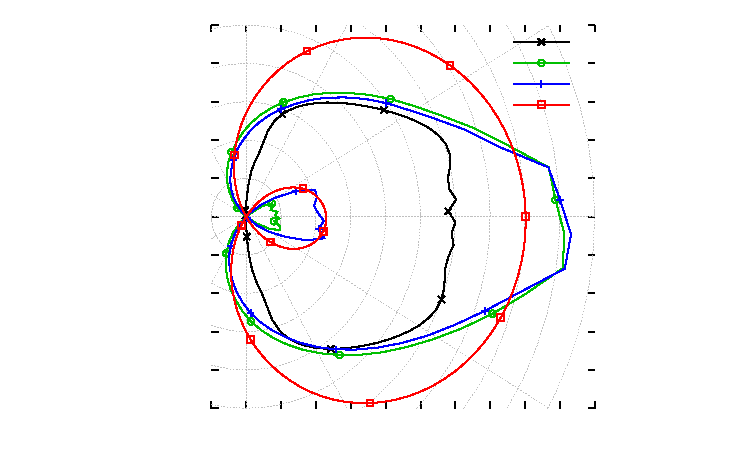
\includegraphics{/Users/seth/_thesis/figures/crashpipe2b/intens-x1-t1/intensity-x1-t1.pdf}}%
    \gplfronttext
  \end{picture}%
\endgroup

  \hspace{-.5in}
  \caption{Scalar flux along the centerline of the channel with a grazing
  boundary condition at $y=0$.}
  \label{fig:bcChannelGrazing}
\end{figure}

A visualization of the angular flux for each method (replacing Monte Carlo with
an \SN\ solution), Fig.~\ref{fig:bcChannelIsotropicAngular}, helps explain the
accuracy
of the AD method and the difference between the reflecting and white boundary
treatments. Even though AD cannot exactly model the peak of freely streaming
photons in the channel (which the \SN\ angular flux shows at $\omega=3\pi/2$),
it accurately approximates the angular flux shape driven by scattering from the
diffusive region (the lobes on the left and right).
The linear-in-angle diffusion approximation cannot represent any of these
features.  

\begin{figure}[htb!]
  \centering\small
  \vspace{-.25in}
  \hspace{-.5in}
  % GNUPLOT: LaTeX picture with Postscript
\begingroup
  \makeatletter
  \providecommand\color[2][]{%
    \GenericError{(gnuplot) \space\space\space\@spaces}{%
      Package color not loaded in conjunction with
      terminal option `colourtext'%
    }{See the gnuplot documentation for explanation.%
    }{Either use 'blacktext' in gnuplot or load the package
      color.sty in LaTeX.}%
    \renewcommand\color[2][]{}%
  }%
  \providecommand\includegraphics[2][]{%
    \GenericError{(gnuplot) \space\space\space\@spaces}{%
      Package graphicx or graphics not loaded%
    }{See the gnuplot documentation for explanation.%
    }{The gnuplot epslatex terminal needs graphicx.sty or graphics.sty.}%
    \renewcommand\includegraphics[2][]{}%
  }%
  \providecommand\rotatebox[2]{#2}%
  \@ifundefined{ifGPcolor}{%
    \newif\ifGPcolor
    \GPcolortrue
  }{}%
  \@ifundefined{ifGPblacktext}{%
    \newif\ifGPblacktext
    \GPblacktexttrue
  }{}%
  % define a \g@addto@macro without @ in the name:
  \let\gplgaddtomacro\g@addto@macro
  % define empty templates for all commands taking text:
  \gdef\gplbacktext{}%
  \gdef\gplfronttext{}%
  \makeatother
  \ifGPblacktext
    % no textcolor at all
    \def\colorrgb#1{}%
    \def\colorgray#1{}%
  \else
    % gray or color?
    \ifGPcolor
      \def\colorrgb#1{\color[rgb]{#1}}%
      \def\colorgray#1{\color[gray]{#1}}%
      \expandafter\def\csname LTw\endcsname{\color{white}}%
      \expandafter\def\csname LTb\endcsname{\color{black}}%
      \expandafter\def\csname LTa\endcsname{\color{black}}%
      \expandafter\def\csname LT0\endcsname{\color[rgb]{1,0,0}}%
      \expandafter\def\csname LT1\endcsname{\color[rgb]{0,1,0}}%
      \expandafter\def\csname LT2\endcsname{\color[rgb]{0,0,1}}%
      \expandafter\def\csname LT3\endcsname{\color[rgb]{1,0,1}}%
      \expandafter\def\csname LT4\endcsname{\color[rgb]{0,1,1}}%
      \expandafter\def\csname LT5\endcsname{\color[rgb]{1,1,0}}%
      \expandafter\def\csname LT6\endcsname{\color[rgb]{0,0,0}}%
      \expandafter\def\csname LT7\endcsname{\color[rgb]{1,0.3,0}}%
      \expandafter\def\csname LT8\endcsname{\color[rgb]{0.5,0.5,0.5}}%
    \else
      % gray
      \def\colorrgb#1{\color{black}}%
      \def\colorgray#1{\color[gray]{#1}}%
      \expandafter\def\csname LTw\endcsname{\color{white}}%
      \expandafter\def\csname LTb\endcsname{\color{black}}%
      \expandafter\def\csname LTa\endcsname{\color{black}}%
      \expandafter\def\csname LT0\endcsname{\color{black}}%
      \expandafter\def\csname LT1\endcsname{\color{black}}%
      \expandafter\def\csname LT2\endcsname{\color{black}}%
      \expandafter\def\csname LT3\endcsname{\color{black}}%
      \expandafter\def\csname LT4\endcsname{\color{black}}%
      \expandafter\def\csname LT5\endcsname{\color{black}}%
      \expandafter\def\csname LT6\endcsname{\color{black}}%
      \expandafter\def\csname LT7\endcsname{\color{black}}%
      \expandafter\def\csname LT8\endcsname{\color{black}}%
    \fi
  \fi
  \setlength{\unitlength}{0.0500bp}%
  \begin{picture}(7200.00,4320.00)%
    \gplgaddtomacro\gplbacktext{%
      \csname LTb\endcsname%
      \put(1910,400){\makebox(0,0)[r]{\strut{} 0.1}}%
      \put(1910,768){\makebox(0,0)[r]{\strut{} 0.08}}%
      \put(1910,1136){\makebox(0,0)[r]{\strut{} 0.06}}%
      \put(1910,1504){\makebox(0,0)[r]{\strut{} 0.04}}%
      \put(1910,1872){\makebox(0,0)[r]{\strut{} 0.02}}%
      \put(1910,2240){\makebox(0,0)[r]{\strut{} 0}}%
      \put(1910,2607){\makebox(0,0)[r]{\strut{} 0.02}}%
      \put(1910,2975){\makebox(0,0)[r]{\strut{} 0.04}}%
      \put(1910,3343){\makebox(0,0)[r]{\strut{} 0.06}}%
      \put(1910,3711){\makebox(0,0)[r]{\strut{} 0.08}}%
      \put(1910,4079){\makebox(0,0)[r]{\strut{} 0.1}}%
      \csname LTb\endcsname%
      \put(2030,200){\makebox(0,0){\strut{} 0.02}}%
      \csname LTb\endcsname%
      \put(2364,200){\makebox(0,0){\strut{} 0}}%
      \csname LTb\endcsname%
      \put(2699,200){\makebox(0,0){\strut{} 0.02}}%
      \csname LTb\endcsname%
      \put(3033,200){\makebox(0,0){\strut{} 0.04}}%
      \csname LTb\endcsname%
      \put(3368,200){\makebox(0,0){\strut{} 0.06}}%
      \csname LTb\endcsname%
      \put(3702,200){\makebox(0,0){\strut{} 0.08}}%
      \csname LTb\endcsname%
      \put(4037,200){\makebox(0,0){\strut{} 0.1}}%
      \csname LTb\endcsname%
      \put(4371,200){\makebox(0,0){\strut{} 0.12}}%
      \csname LTb\endcsname%
      \put(4706,200){\makebox(0,0){\strut{} 0.14}}%
      \csname LTb\endcsname%
      \put(5040,200){\makebox(0,0){\strut{} 0.16}}%
      \csname LTb\endcsname%
      \put(5375,200){\makebox(0,0){\strut{} 0.18}}%
      \csname LTb\endcsname%
      \put(5709,200){\makebox(0,0){\strut{} 0.2}}%
      \csname LTb\endcsname%
      \put(1330,2239){\rotatebox{-270}{\makebox(0,0){\strut{}x1 center $(1.01,3.5)$}}}%
    }%
    \gplgaddtomacro\gplfronttext{%
      \csname LTb\endcsname%
      \put(4806,3916){\makebox(0,0)[r]{\strut{}S$_{128}$}}%
      \csname LTb\endcsname%
      \put(4806,3716){\makebox(0,0)[r]{\strut{}FLAD$_{64}$}}%
      \csname LTb\endcsname%
      \put(4806,3516){\makebox(0,0)[r]{\strut{}AD$_{64}$}}%
      \csname LTb\endcsname%
      \put(4806,3316){\makebox(0,0)[r]{\strut{}FLD}}%
    }%
    \gplbacktext
    \put(0,0){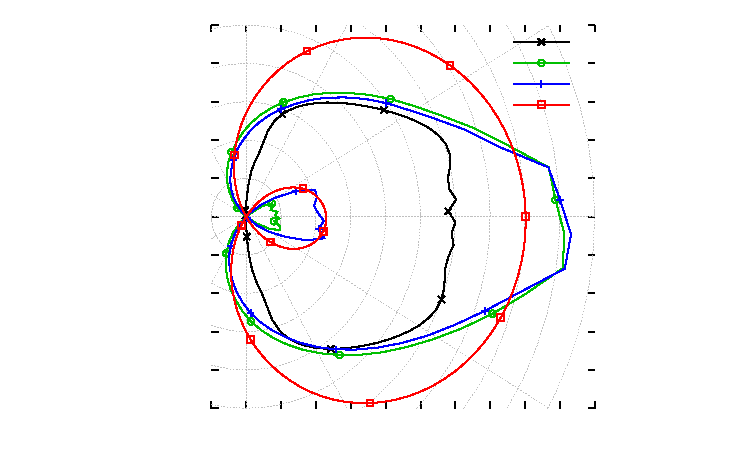
\includegraphics{/Users/seth/_thesis/figures/crashpipe2b/intens-x1-t1/intensity-x1-t1.pdf}}%
    \gplfronttext
  \end{picture}%
\endgroup

  \hspace{-.5in}
  \vspace{-.25in}
  \caption{Angular flux $\psi(2.5, 1., \omega)$ for the incident isotropic
  problem, in the centerline of the channel one unit from the boundary.}
  \label{fig:bcChannelIsotropicAngular}
\end{figure}

The shape around $\omega=\pi/2$ gives insight into why the white boundary
performs better in this problem: a reflecting boundary produces a peak in $f$
along the channel, but a white boundary gives a more isotropic shape near that
range, better matching the incident isotropic boundary condition. This suggests
that the qualitatively best way to satisfy Eq.~\eqref{eq:zetaCondition1} may be
to have $\zeta$ take the shape of the true boundary condition.

%%%%%%%%%%%%%%%%%%%%%%%%%%%%%%%%%%%%%%%%%%%%%%%%%%%%%%%%%%%%%%%%%%%%%%%%%%%%%%%%
\clearpage
\subsection{Steady-state flatland checkers}

Here we consider a difficult problem that has repeating variations in both $x$
and $y$ directions. It uses $c=0.99$, 

The anisotropic diffusion coefficients are plotted as ellipses in
Fig.~\ref{fig:bcCheckersAdcoeff}. The major axis is along the principal
eigenvector of the diffusion tensor and is in length proportional to the
principal eigenvalue; the more isotropic the tensor, the more circular the
glyph. Red and larger ellipses represent larger AD coefficients.

\begin{figure}[htb]
  \centering\small
  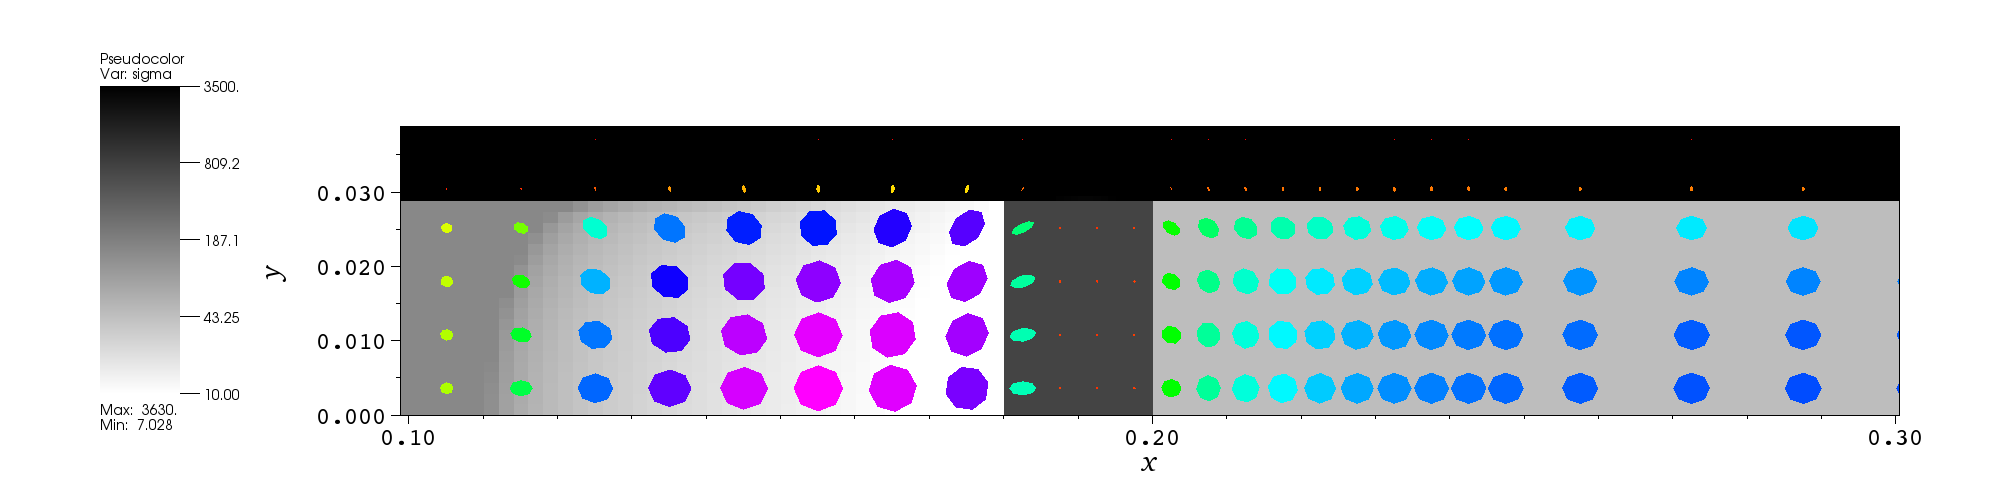
\includegraphics[width=3in]{adbc-checkers/adcoeff}
  \caption[Anisotropic diffusion coefficients for the checker problem.]{
  Anisotropic diffusion coefficients for the checker problem. Dark
  regions have $\sigma=1$, light regions have $\sigma=0.01$.}
  \label{fig:bcCheckersAdcoeff}
\end{figure}

\begin{figure}[htb]
  \centering\small
  \hspace{-.5in}
  % GNUPLOT: LaTeX picture with Postscript
\begingroup
  \makeatletter
  \providecommand\color[2][]{%
    \GenericError{(gnuplot) \space\space\space\@spaces}{%
      Package color not loaded in conjunction with
      terminal option `colourtext'%
    }{See the gnuplot documentation for explanation.%
    }{Either use 'blacktext' in gnuplot or load the package
      color.sty in LaTeX.}%
    \renewcommand\color[2][]{}%
  }%
  \providecommand\includegraphics[2][]{%
    \GenericError{(gnuplot) \space\space\space\@spaces}{%
      Package graphicx or graphics not loaded%
    }{See the gnuplot documentation for explanation.%
    }{The gnuplot epslatex terminal needs graphicx.sty or graphics.sty.}%
    \renewcommand\includegraphics[2][]{}%
  }%
  \providecommand\rotatebox[2]{#2}%
  \@ifundefined{ifGPcolor}{%
    \newif\ifGPcolor
    \GPcolortrue
  }{}%
  \@ifundefined{ifGPblacktext}{%
    \newif\ifGPblacktext
    \GPblacktexttrue
  }{}%
  % define a \g@addto@macro without @ in the name:
  \let\gplgaddtomacro\g@addto@macro
  % define empty templates for all commands taking text:
  \gdef\gplbacktext{}%
  \gdef\gplfronttext{}%
  \makeatother
  \ifGPblacktext
    % no textcolor at all
    \def\colorrgb#1{}%
    \def\colorgray#1{}%
  \else
    % gray or color?
    \ifGPcolor
      \def\colorrgb#1{\color[rgb]{#1}}%
      \def\colorgray#1{\color[gray]{#1}}%
      \expandafter\def\csname LTw\endcsname{\color{white}}%
      \expandafter\def\csname LTb\endcsname{\color{black}}%
      \expandafter\def\csname LTa\endcsname{\color{black}}%
      \expandafter\def\csname LT0\endcsname{\color[rgb]{1,0,0}}%
      \expandafter\def\csname LT1\endcsname{\color[rgb]{0,1,0}}%
      \expandafter\def\csname LT2\endcsname{\color[rgb]{0,0,1}}%
      \expandafter\def\csname LT3\endcsname{\color[rgb]{1,0,1}}%
      \expandafter\def\csname LT4\endcsname{\color[rgb]{0,1,1}}%
      \expandafter\def\csname LT5\endcsname{\color[rgb]{1,1,0}}%
      \expandafter\def\csname LT6\endcsname{\color[rgb]{0,0,0}}%
      \expandafter\def\csname LT7\endcsname{\color[rgb]{1,0.3,0}}%
      \expandafter\def\csname LT8\endcsname{\color[rgb]{0.5,0.5,0.5}}%
    \else
      % gray
      \def\colorrgb#1{\color{black}}%
      \def\colorgray#1{\color[gray]{#1}}%
      \expandafter\def\csname LTw\endcsname{\color{white}}%
      \expandafter\def\csname LTb\endcsname{\color{black}}%
      \expandafter\def\csname LTa\endcsname{\color{black}}%
      \expandafter\def\csname LT0\endcsname{\color{black}}%
      \expandafter\def\csname LT1\endcsname{\color{black}}%
      \expandafter\def\csname LT2\endcsname{\color{black}}%
      \expandafter\def\csname LT3\endcsname{\color{black}}%
      \expandafter\def\csname LT4\endcsname{\color{black}}%
      \expandafter\def\csname LT5\endcsname{\color{black}}%
      \expandafter\def\csname LT6\endcsname{\color{black}}%
      \expandafter\def\csname LT7\endcsname{\color{black}}%
      \expandafter\def\csname LT8\endcsname{\color{black}}%
    \fi
  \fi
  \setlength{\unitlength}{0.0500bp}%
  \begin{picture}(7200.00,4320.00)%
    \gplgaddtomacro\gplbacktext{%
      \csname LTb\endcsname%
      \put(1910,400){\makebox(0,0)[r]{\strut{} 0.1}}%
      \put(1910,768){\makebox(0,0)[r]{\strut{} 0.08}}%
      \put(1910,1136){\makebox(0,0)[r]{\strut{} 0.06}}%
      \put(1910,1504){\makebox(0,0)[r]{\strut{} 0.04}}%
      \put(1910,1872){\makebox(0,0)[r]{\strut{} 0.02}}%
      \put(1910,2240){\makebox(0,0)[r]{\strut{} 0}}%
      \put(1910,2607){\makebox(0,0)[r]{\strut{} 0.02}}%
      \put(1910,2975){\makebox(0,0)[r]{\strut{} 0.04}}%
      \put(1910,3343){\makebox(0,0)[r]{\strut{} 0.06}}%
      \put(1910,3711){\makebox(0,0)[r]{\strut{} 0.08}}%
      \put(1910,4079){\makebox(0,0)[r]{\strut{} 0.1}}%
      \csname LTb\endcsname%
      \put(2030,200){\makebox(0,0){\strut{} 0.02}}%
      \csname LTb\endcsname%
      \put(2364,200){\makebox(0,0){\strut{} 0}}%
      \csname LTb\endcsname%
      \put(2699,200){\makebox(0,0){\strut{} 0.02}}%
      \csname LTb\endcsname%
      \put(3033,200){\makebox(0,0){\strut{} 0.04}}%
      \csname LTb\endcsname%
      \put(3368,200){\makebox(0,0){\strut{} 0.06}}%
      \csname LTb\endcsname%
      \put(3702,200){\makebox(0,0){\strut{} 0.08}}%
      \csname LTb\endcsname%
      \put(4037,200){\makebox(0,0){\strut{} 0.1}}%
      \csname LTb\endcsname%
      \put(4371,200){\makebox(0,0){\strut{} 0.12}}%
      \csname LTb\endcsname%
      \put(4706,200){\makebox(0,0){\strut{} 0.14}}%
      \csname LTb\endcsname%
      \put(5040,200){\makebox(0,0){\strut{} 0.16}}%
      \csname LTb\endcsname%
      \put(5375,200){\makebox(0,0){\strut{} 0.18}}%
      \csname LTb\endcsname%
      \put(5709,200){\makebox(0,0){\strut{} 0.2}}%
      \csname LTb\endcsname%
      \put(1330,2239){\rotatebox{-270}{\makebox(0,0){\strut{}x1 center $(1.01,3.5)$}}}%
    }%
    \gplgaddtomacro\gplfronttext{%
      \csname LTb\endcsname%
      \put(4806,3916){\makebox(0,0)[r]{\strut{}S$_{128}$}}%
      \csname LTb\endcsname%
      \put(4806,3716){\makebox(0,0)[r]{\strut{}FLAD$_{64}$}}%
      \csname LTb\endcsname%
      \put(4806,3516){\makebox(0,0)[r]{\strut{}AD$_{64}$}}%
      \csname LTb\endcsname%
      \put(4806,3316){\makebox(0,0)[r]{\strut{}FLD}}%
    }%
    \gplbacktext
    \put(0,0){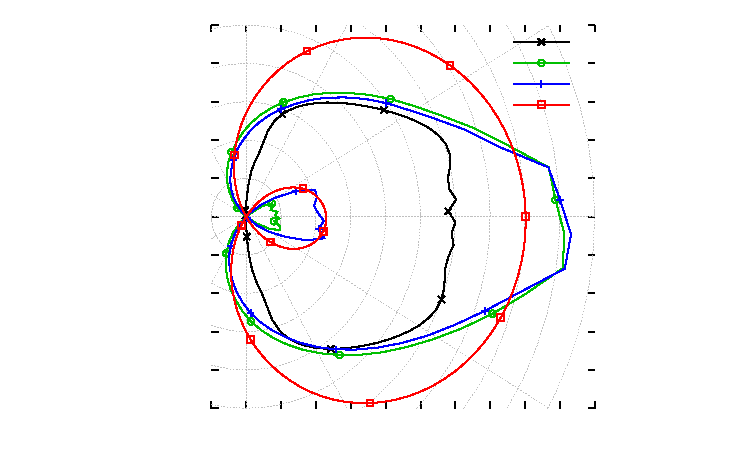
\includegraphics{/Users/seth/_thesis/figures/crashpipe2b/intens-x1-t1/intensity-x1-t1.pdf}}%
    \gplfronttext
  \end{picture}%
\endgroup

  \hspace{-.5in}
  \caption{Scalar flux along $x=2$ of the checker problem with an isotropic
  boundary condition at $y=0$.}
  \label{fig:bcCheckersIsotropic}
\end{figure}

\begin{figure}[htb]
  \centering\small
  \hspace{-.5in}
  % GNUPLOT: LaTeX picture with Postscript
\begingroup
  \makeatletter
  \providecommand\color[2][]{%
    \GenericError{(gnuplot) \space\space\space\@spaces}{%
      Package color not loaded in conjunction with
      terminal option `colourtext'%
    }{See the gnuplot documentation for explanation.%
    }{Either use 'blacktext' in gnuplot or load the package
      color.sty in LaTeX.}%
    \renewcommand\color[2][]{}%
  }%
  \providecommand\includegraphics[2][]{%
    \GenericError{(gnuplot) \space\space\space\@spaces}{%
      Package graphicx or graphics not loaded%
    }{See the gnuplot documentation for explanation.%
    }{The gnuplot epslatex terminal needs graphicx.sty or graphics.sty.}%
    \renewcommand\includegraphics[2][]{}%
  }%
  \providecommand\rotatebox[2]{#2}%
  \@ifundefined{ifGPcolor}{%
    \newif\ifGPcolor
    \GPcolortrue
  }{}%
  \@ifundefined{ifGPblacktext}{%
    \newif\ifGPblacktext
    \GPblacktexttrue
  }{}%
  % define a \g@addto@macro without @ in the name:
  \let\gplgaddtomacro\g@addto@macro
  % define empty templates for all commands taking text:
  \gdef\gplbacktext{}%
  \gdef\gplfronttext{}%
  \makeatother
  \ifGPblacktext
    % no textcolor at all
    \def\colorrgb#1{}%
    \def\colorgray#1{}%
  \else
    % gray or color?
    \ifGPcolor
      \def\colorrgb#1{\color[rgb]{#1}}%
      \def\colorgray#1{\color[gray]{#1}}%
      \expandafter\def\csname LTw\endcsname{\color{white}}%
      \expandafter\def\csname LTb\endcsname{\color{black}}%
      \expandafter\def\csname LTa\endcsname{\color{black}}%
      \expandafter\def\csname LT0\endcsname{\color[rgb]{1,0,0}}%
      \expandafter\def\csname LT1\endcsname{\color[rgb]{0,1,0}}%
      \expandafter\def\csname LT2\endcsname{\color[rgb]{0,0,1}}%
      \expandafter\def\csname LT3\endcsname{\color[rgb]{1,0,1}}%
      \expandafter\def\csname LT4\endcsname{\color[rgb]{0,1,1}}%
      \expandafter\def\csname LT5\endcsname{\color[rgb]{1,1,0}}%
      \expandafter\def\csname LT6\endcsname{\color[rgb]{0,0,0}}%
      \expandafter\def\csname LT7\endcsname{\color[rgb]{1,0.3,0}}%
      \expandafter\def\csname LT8\endcsname{\color[rgb]{0.5,0.5,0.5}}%
    \else
      % gray
      \def\colorrgb#1{\color{black}}%
      \def\colorgray#1{\color[gray]{#1}}%
      \expandafter\def\csname LTw\endcsname{\color{white}}%
      \expandafter\def\csname LTb\endcsname{\color{black}}%
      \expandafter\def\csname LTa\endcsname{\color{black}}%
      \expandafter\def\csname LT0\endcsname{\color{black}}%
      \expandafter\def\csname LT1\endcsname{\color{black}}%
      \expandafter\def\csname LT2\endcsname{\color{black}}%
      \expandafter\def\csname LT3\endcsname{\color{black}}%
      \expandafter\def\csname LT4\endcsname{\color{black}}%
      \expandafter\def\csname LT5\endcsname{\color{black}}%
      \expandafter\def\csname LT6\endcsname{\color{black}}%
      \expandafter\def\csname LT7\endcsname{\color{black}}%
      \expandafter\def\csname LT8\endcsname{\color{black}}%
    \fi
  \fi
  \setlength{\unitlength}{0.0500bp}%
  \begin{picture}(7200.00,4320.00)%
    \gplgaddtomacro\gplbacktext{%
      \csname LTb\endcsname%
      \put(1910,400){\makebox(0,0)[r]{\strut{} 0.1}}%
      \put(1910,768){\makebox(0,0)[r]{\strut{} 0.08}}%
      \put(1910,1136){\makebox(0,0)[r]{\strut{} 0.06}}%
      \put(1910,1504){\makebox(0,0)[r]{\strut{} 0.04}}%
      \put(1910,1872){\makebox(0,0)[r]{\strut{} 0.02}}%
      \put(1910,2240){\makebox(0,0)[r]{\strut{} 0}}%
      \put(1910,2607){\makebox(0,0)[r]{\strut{} 0.02}}%
      \put(1910,2975){\makebox(0,0)[r]{\strut{} 0.04}}%
      \put(1910,3343){\makebox(0,0)[r]{\strut{} 0.06}}%
      \put(1910,3711){\makebox(0,0)[r]{\strut{} 0.08}}%
      \put(1910,4079){\makebox(0,0)[r]{\strut{} 0.1}}%
      \csname LTb\endcsname%
      \put(2030,200){\makebox(0,0){\strut{} 0.02}}%
      \csname LTb\endcsname%
      \put(2364,200){\makebox(0,0){\strut{} 0}}%
      \csname LTb\endcsname%
      \put(2699,200){\makebox(0,0){\strut{} 0.02}}%
      \csname LTb\endcsname%
      \put(3033,200){\makebox(0,0){\strut{} 0.04}}%
      \csname LTb\endcsname%
      \put(3368,200){\makebox(0,0){\strut{} 0.06}}%
      \csname LTb\endcsname%
      \put(3702,200){\makebox(0,0){\strut{} 0.08}}%
      \csname LTb\endcsname%
      \put(4037,200){\makebox(0,0){\strut{} 0.1}}%
      \csname LTb\endcsname%
      \put(4371,200){\makebox(0,0){\strut{} 0.12}}%
      \csname LTb\endcsname%
      \put(4706,200){\makebox(0,0){\strut{} 0.14}}%
      \csname LTb\endcsname%
      \put(5040,200){\makebox(0,0){\strut{} 0.16}}%
      \csname LTb\endcsname%
      \put(5375,200){\makebox(0,0){\strut{} 0.18}}%
      \csname LTb\endcsname%
      \put(5709,200){\makebox(0,0){\strut{} 0.2}}%
      \csname LTb\endcsname%
      \put(1330,2239){\rotatebox{-270}{\makebox(0,0){\strut{}x1 center $(1.01,3.5)$}}}%
    }%
    \gplgaddtomacro\gplfronttext{%
      \csname LTb\endcsname%
      \put(4806,3916){\makebox(0,0)[r]{\strut{}S$_{128}$}}%
      \csname LTb\endcsname%
      \put(4806,3716){\makebox(0,0)[r]{\strut{}FLAD$_{64}$}}%
      \csname LTb\endcsname%
      \put(4806,3516){\makebox(0,0)[r]{\strut{}AD$_{64}$}}%
      \csname LTb\endcsname%
      \put(4806,3316){\makebox(0,0)[r]{\strut{}FLD}}%
    }%
    \gplbacktext
    \put(0,0){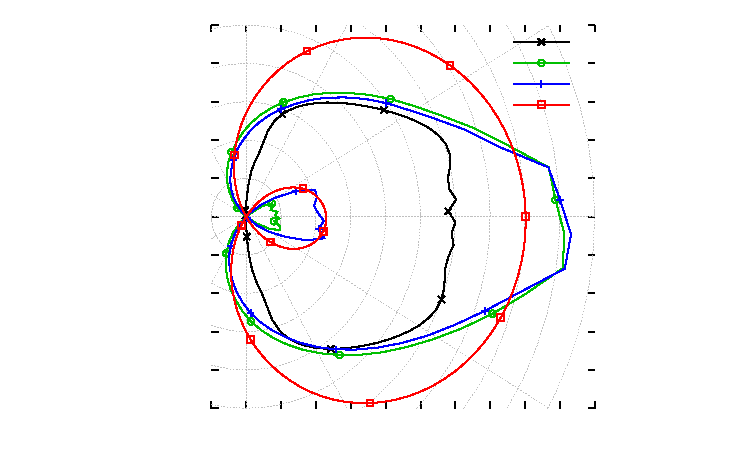
\includegraphics{/Users/seth/_thesis/figures/crashpipe2b/intens-x1-t1/intensity-x1-t1.pdf}}%
    \gplfronttext
  \end{picture}%
\endgroup

  \hspace{-.5in}
  \caption{Scalar flux along $x=2$ of the checker problem with a normal
  boundary condition at $y=0$.}
  \label{fig:bcCheckersDelta}
\end{figure}

%%%%%%%%%%%%%%%%%%%%%%%%%%%%%%%%%%%%%%%%%%%%%%%%%%%%%%%%%%%%%%%%%%%%%%%%%%%%%%%%
\section{Linear time-dependent behavior}

Before considering the complex nonlinear behavior of TRT, we should
independently analyze how the newly developed methods behave in linear,
time-dependent problems with time-independent opacities.

\subsection{Blast wave}

Ran a test problem inside a channel with a ``blast wave'' initial condition. It
resides in $0 \le x \le 3$, $-1.1 \le y \le 1.1$, with a thin region inside
$-.1 \le y \le .1$. It has reflecting boundary conditions everywhere.

The initial condition is
\begin{equation*}
  \phi(x,y) = 0.001 + a \eexp^{-100 (x^2 + y^2) }
\end{equation*}
where $a$ is a normalization constant that gives a total initial $\int \phi
\ud V$ of $100 + 0.001 V$. We use $\sigma=1$ inside the channel, $\sigma=10$
outside, $c=0.99$ everywhere.

